\documentclass[twoside]{book}

% Packages required by doxygen
\usepackage{calc}
\usepackage{doxygen}
\usepackage{graphicx}
\usepackage[utf8]{inputenc}
\usepackage{makeidx}
\usepackage{multicol}
\usepackage{multirow}
\usepackage{textcomp}
\usepackage[table]{xcolor}

% Font selection
\usepackage[T1]{fontenc}
\usepackage{mathptmx}
\usepackage[scaled=.90]{helvet}
\usepackage{courier}
\usepackage{amssymb}
\usepackage{sectsty}
\renewcommand{\familydefault}{\sfdefault}
\allsectionsfont{%
  \fontseries{bc}\selectfont%
  \color{darkgray}%
}
\renewcommand{\DoxyLabelFont}{%
  \fontseries{bc}\selectfont%
  \color{darkgray}%
}

% Page & text layout
\usepackage{geometry}
\geometry{%
  a4paper,%
  top=2.5cm,%
  bottom=2.5cm,%
  left=2.5cm,%
  right=2.5cm%
}
\tolerance=750
\hfuzz=15pt
\hbadness=750
\setlength{\emergencystretch}{15pt}
\setlength{\parindent}{0cm}
\setlength{\parskip}{0.2cm}
\makeatletter
\renewcommand{\paragraph}{%
  \@startsection{paragraph}{4}{0ex}{-1.0ex}{1.0ex}{%
    \normalfont\normalsize\bfseries\SS@parafont%
  }%
}
\renewcommand{\subparagraph}{%
  \@startsection{subparagraph}{5}{0ex}{-1.0ex}{1.0ex}{%
    \normalfont\normalsize\bfseries\SS@subparafont%
  }%
}
\makeatother

% Headers & footers
\usepackage{fancyhdr}
\pagestyle{fancyplain}
\fancyhead[LE]{\fancyplain{}{\bfseries\thepage}}
\fancyhead[CE]{\fancyplain{}{}}
\fancyhead[RE]{\fancyplain{}{\bfseries\leftmark}}
\fancyhead[LO]{\fancyplain{}{\bfseries\rightmark}}
\fancyhead[CO]{\fancyplain{}{}}
\fancyhead[RO]{\fancyplain{}{\bfseries\thepage}}
\fancyfoot[LE]{\fancyplain{}{}}
\fancyfoot[CE]{\fancyplain{}{}}
\fancyfoot[RE]{\fancyplain{}{\bfseries\scriptsize Generated on Thu Apr 3 2014 14\-:49\-:22 for Trans\-Amercia by Doxygen }}
\fancyfoot[LO]{\fancyplain{}{\bfseries\scriptsize Generated on Thu Apr 3 2014 14\-:49\-:22 for Trans\-Amercia by Doxygen }}
\fancyfoot[CO]{\fancyplain{}{}}
\fancyfoot[RO]{\fancyplain{}{}}
\renewcommand{\footrulewidth}{0.4pt}
\renewcommand{\chaptermark}[1]{%
  \markboth{#1}{}%
}
\renewcommand{\sectionmark}[1]{%
  \markright{\thesection\ #1}%
}

% Indices & bibliography
\usepackage{natbib}
\usepackage[titles]{tocloft}
\setcounter{tocdepth}{3}
\setcounter{secnumdepth}{5}
\makeindex

% Custom commands
\newcommand{\clearemptydoublepage}{%
  \newpage{\pagestyle{empty}\cleardoublepage}%
}


%===== C O N T E N T S =====

\begin{document}

% Titlepage & ToC
\pagenumbering{roman}
\begin{titlepage}
\vspace*{7cm}
\begin{center}%
{\Large Trans\-Amercia \\[1ex]\large v0.\-4 }\\
\vspace*{1cm}
{\large Generated by Doxygen 1.8.6}\\
\vspace*{0.5cm}
{\small Thu Apr 3 2014 14:49:22}\\
\end{center}
\end{titlepage}
\clearemptydoublepage
\tableofcontents
\clearemptydoublepage
\pagenumbering{arabic}

%--- Begin generated contents ---
\chapter{Hierarchical Index}
\section{Class Hierarchy}
This inheritance list is sorted roughly, but not completely, alphabetically\-:\begin{DoxyCompactList}
\item \contentsline{section}{A\-I}{\pageref{class_a_i}}{}
\begin{DoxyCompactList}
\item \contentsline{section}{test\-K\-I}{\pageref{classtest_k_i}}{}
\end{DoxyCompactList}
\item \contentsline{section}{Board}{\pageref{class_board}}{}
\item \contentsline{section}{Connection}{\pageref{class_connection}}{}
\item \contentsline{section}{Counter}{\pageref{class_counter}}{}
\item \contentsline{section}{Game}{\pageref{class_game}}{}
\item \contentsline{section}{Game\-Logger}{\pageref{class_game_logger}}{}
\item \contentsline{section}{Playing\-Order\-:\-:iterator}{\pageref{class_playing_order_1_1iterator}}{}
\item \contentsline{section}{Move}{\pageref{class_move}}{}
\item \contentsline{section}{Playing\-Order}{\pageref{class_playing_order}}{}
\item Q\-Dialog\begin{DoxyCompactList}
\item \contentsline{section}{Initialize}{\pageref{class_initialize}}{}
\end{DoxyCompactList}
\item Q\-Main\-Window\begin{DoxyCompactList}
\item \contentsline{section}{Main\-Window}{\pageref{class_main_window}}{}
\end{DoxyCompactList}
\item Q\-Widget\begin{DoxyCompactList}
\item \contentsline{section}{Spielbrett}{\pageref{class_spielbrett}}{}
\item \contentsline{section}{Window}{\pageref{class_window}}{}
\end{DoxyCompactList}
\item \contentsline{section}{Round}{\pageref{class_round}}{}
\item \contentsline{section}{Round\-Logger}{\pageref{class_round_logger}}{}
\item \contentsline{section}{Simulation}{\pageref{class_simulation}}{}
\item \contentsline{section}{Simulation\-Logger}{\pageref{class_simulation_logger}}{}
\item \contentsline{section}{State}{\pageref{class_state}}{}
\item \contentsline{section}{U\-I\-E\-X\-E\-C}{\pageref{class_u_i_e_x_e_c}}{}
\item \contentsline{section}{Vector}{\pageref{class_vector}}{}
\begin{DoxyCompactList}
\item \contentsline{section}{City}{\pageref{class_city}}{}
\item \contentsline{section}{Coordinate}{\pageref{class_coordinate}}{}
\item \contentsline{section}{Pawn}{\pageref{class_pawn}}{}
\end{DoxyCompactList}
\end{DoxyCompactList}

\chapter{Class Index}
\section{Class List}
Here are the classes, structs, unions and interfaces with brief descriptions\-:\begin{DoxyCompactList}
\item\contentsline{section}{{\bf A\-I} }{\pageref{class_a_i}}{}
\item\contentsline{section}{{\bf Board} }{\pageref{class_board}}{}
\item\contentsline{section}{{\bf City} }{\pageref{class_city}}{}
\item\contentsline{section}{{\bf Connection} }{\pageref{class_connection}}{}
\item\contentsline{section}{{\bf Coordinate} }{\pageref{class_coordinate}}{}
\item\contentsline{section}{{\bf Counter} }{\pageref{class_counter}}{}
\item\contentsline{section}{{\bf Dynamic\-State} }{\pageref{class_dynamic_state}}{}
\item\contentsline{section}{{\bf Game} }{\pageref{class_game}}{}
\item\contentsline{section}{{\bf Game\-Logger} }{\pageref{class_game_logger}}{}
\item\contentsline{section}{{\bf Initialize} }{\pageref{class_initialize}}{}
\item\contentsline{section}{{\bf Playing\-Order\-::iterator} }{\pageref{class_playing_order_1_1iterator}}{}
\item\contentsline{section}{{\bf Main\-Window} }{\pageref{class_main_window}}{}
\item\contentsline{section}{{\bf Move} }{\pageref{class_move}}{}
\item\contentsline{section}{{\bf Pawn} }{\pageref{class_pawn}}{}
\item\contentsline{section}{{\bf Playing\-Order} }{\pageref{class_playing_order}}{}
\item\contentsline{section}{{\bf Round} }{\pageref{class_round}}{}
\item\contentsline{section}{{\bf Round\-Logger} }{\pageref{class_round_logger}}{}
\item\contentsline{section}{{\bf Simulation} }{\pageref{class_simulation}}{}
\item\contentsline{section}{{\bf Simulation\-Logger} }{\pageref{class_simulation_logger}}{}
\item\contentsline{section}{{\bf Spielbrett} }{\pageref{class_spielbrett}}{}
\item\contentsline{section}{{\bf State} }{\pageref{class_state}}{}
\item\contentsline{section}{{\bf test\-K\-I} }{\pageref{classtest_k_i}}{}
\item\contentsline{section}{{\bf U\-I\-E\-X\-E\-C} }{\pageref{class_u_i_e_x_e_c}}{}
\item\contentsline{section}{{\bf Vector} }{\pageref{class_vector}}{}
\item\contentsline{section}{{\bf Window} }{\pageref{class_window}}{}
\end{DoxyCompactList}

\chapter{Class Documentation}
\section{A\-I Class Reference}
\label{class_a_i}\index{A\-I@{A\-I}}


{\ttfamily \#include $<$A\-I.\-h$>$}

Inheritance diagram for A\-I\-:\begin{figure}[H]
\begin{center}
\leavevmode
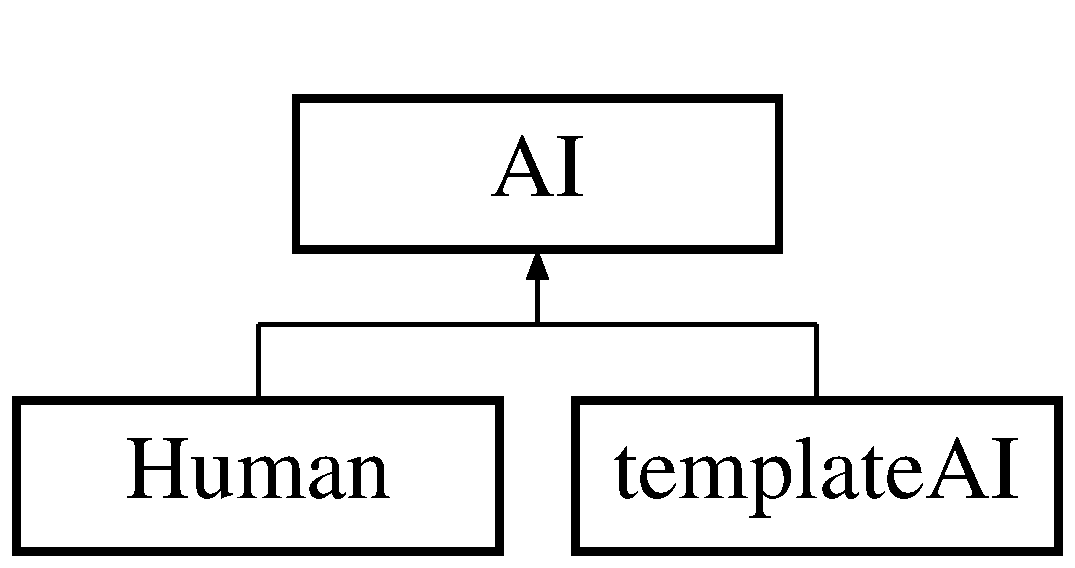
\includegraphics[height=2.000000cm]{class_a_i}
\end{center}
\end{figure}
\subsection*{Public Member Functions}
\begin{DoxyCompactItemize}
\item 
{\bf A\-I} (P\-L\-A\-Y\-E\-R\-C\-O\-L\-O\-R {\bf player\-Color})
\end{DoxyCompactItemize}
\subsection*{Public Attributes}
\begin{DoxyCompactItemize}
\item 
const P\-L\-A\-Y\-E\-R\-C\-O\-L\-O\-R {\bf player\-Color}
\item 
string {\bf owner}
\item 
string {\bf A\-Iname}
\end{DoxyCompactItemize}
\subsection*{Protected Member Functions}
\begin{DoxyCompactItemize}
\item 
virtual {\bf Move} {\bf do\-Move} ({\bf State} \&aktuell, vector$<$ {\bf Move} $\ast$ $>$ move\-List)=0
\item 
virtual const {\bf Coordinate} $\ast$ {\bf set\-Pawn} ({\bf State} \&aktuell)=0
\item 
virtual bool {\bf count\-Points} ({\bf State} \&current\-State, vector$<$ {\bf Connection} $\ast$ $>$ \&return\-Path)=0
\item 
virtual void {\bf gather\-Information\-End\-Of\-Round} (const {\bf Round\-Logger} $\ast$current\-Infos)=0
\end{DoxyCompactItemize}
\subsection*{Protected Attributes}
\begin{DoxyCompactItemize}
\item 
const {\bf City} $\ast$$\ast$ {\bf hand}
\end{DoxyCompactItemize}
\subsection*{Friends}
\begin{DoxyCompactItemize}
\item 
class {\bfseries Game}\label{class_a_i_aa2fab026580d6f14280c2ffb8063a314}

\item 
class {\bfseries Round}\label{class_a_i_aae72f8e1249fbf187032c257b544873d}

\end{DoxyCompactItemize}


\subsection{Detailed Description}
If you want to create your own \doxyref{A\-I}{p.}{class_a_i}, you have to implement this class as a kind of interface. You have to implement every abstract method. 

\subsection{Constructor \& Destructor Documentation}
\index{A\-I@{A\-I}!A\-I@{A\-I}}
\index{A\-I@{A\-I}!AI@{A\-I}}
\subsubsection[{A\-I}]{\setlength{\rightskip}{0pt plus 5cm}A\-I\-::\-A\-I (
\begin{DoxyParamCaption}
\item[{P\-L\-A\-Y\-E\-R\-C\-O\-L\-O\-R}]{player\-Color}
\end{DoxyParamCaption}
)}\label{class_a_i_af4f94640ca8c67c79c085a4cd81a2f51}
A constructor where you can set the name of your \doxyref{A\-I}{p.}{class_a_i} and your name, but not much more ;) 

\subsection{Member Function Documentation}
\index{A\-I@{A\-I}!count\-Points@{count\-Points}}
\index{count\-Points@{count\-Points}!AI@{A\-I}}
\subsubsection[{count\-Points}]{\setlength{\rightskip}{0pt plus 5cm}virtual bool A\-I\-::count\-Points (
\begin{DoxyParamCaption}
\item[{{\bf State} \&}]{current\-State, }
\item[{vector$<$ {\bf Connection} $\ast$ $>$ \&}]{return\-Path}
\end{DoxyParamCaption}
)\hspace{0.3cm}{\ttfamily [protected]}, {\ttfamily [pure virtual]}}\label{class_a_i_a158672aaf98fab1b1ede48002f83d3ff}
Here you can count your minus points at the end of each round. If you want to do so, you have to return true. For the beginning it is okay, if you just return false. Then the gamemaster will count the minuspoints. He counts in most cases the minimum of minuspoints you get, however in some cases the algorithm doesn't evaluate the best value. 

Implemented in {\bf debugger\-A\-I} \doxyref{}{p.}{classdebugger_a_i_a4eae0a3715a66df1e9773a0bb8851318}, {\bf template\-A\-I} \doxyref{}{p.}{classtemplate_a_i_a254a3e1a7a2cd1d16bec816cb9fab075}, {\bf David\-A\-I} \doxyref{}{p.}{class_david_a_i_afcc7dbeec6565efdaf1dd25559d536ca}, {\bf test\-K\-I} \doxyref{}{p.}{classtest_k_i_a76d7f00e5e5464c34bb2ad5e9062abf9}, and {\bf Human} \doxyref{}{p.}{class_human_a1d9b69f7ac17c8ead5d78e5af312250a}.

\index{A\-I@{A\-I}!do\-Move@{do\-Move}}
\index{do\-Move@{do\-Move}!AI@{A\-I}}
\subsubsection[{do\-Move}]{\setlength{\rightskip}{0pt plus 5cm}virtual {\bf Move} A\-I\-::do\-Move (
\begin{DoxyParamCaption}
\item[{{\bf State} \&}]{aktuell, }
\item[{vector$<$ {\bf Move} $\ast$ $>$}]{move\-List}
\end{DoxyParamCaption}
)\hspace{0.3cm}{\ttfamily [protected]}, {\ttfamily [pure virtual]}}\label{class_a_i_ade352ac8d216d67feca731a127b50e6f}
Inside this methode you calculate your next move in the game. 

Implemented in {\bf debugger\-A\-I} \doxyref{}{p.}{classdebugger_a_i_a6948d2ae193d1086955b71efe3a87de1}, {\bf template\-A\-I} \doxyref{}{p.}{classtemplate_a_i_a9abd9bfabeb26ba77ed5090cb1716a2a}, {\bf David\-A\-I} \doxyref{}{p.}{class_david_a_i_a66501d9cbc5972a6fc237a87774a9425}, {\bf test\-K\-I} \doxyref{}{p.}{classtest_k_i_a195ad45b09daced4e650ce228f4da8f3}, and {\bf Human} \doxyref{}{p.}{class_human_a797f11c25934d3e6ebdfa612715f899a}.

\index{A\-I@{A\-I}!gather\-Information\-End\-Of\-Round@{gather\-Information\-End\-Of\-Round}}
\index{gather\-Information\-End\-Of\-Round@{gather\-Information\-End\-Of\-Round}!AI@{A\-I}}
\subsubsection[{gather\-Information\-End\-Of\-Round}]{\setlength{\rightskip}{0pt plus 5cm}virtual void A\-I\-::gather\-Information\-End\-Of\-Round (
\begin{DoxyParamCaption}
\item[{const {\bf Round\-Logger} $\ast$}]{current\-Infos}
\end{DoxyParamCaption}
)\hspace{0.3cm}{\ttfamily [protected]}, {\ttfamily [pure virtual]}}\label{class_a_i_a8565a9ef04ac4f9913913c99f65213b2}
At the end of each round you can take a look at the whole game and the playing cards of your opponents. This can be usefull, if you want to figure out there strategy and react to that over a simulation period. 

Implemented in {\bf debugger\-A\-I} \doxyref{}{p.}{classdebugger_a_i_ab90bbce673b55483d6156dea09726952}, {\bf template\-A\-I} \doxyref{}{p.}{classtemplate_a_i_acfc0b92fbecc56c0dbde089c350f99e5}, {\bf David\-A\-I} \doxyref{}{p.}{class_david_a_i_a160ac3d032a3b6afb77f693ca3d5c8b6}, {\bf test\-K\-I} \doxyref{}{p.}{classtest_k_i_a84b8e65aca959d95d89d80194e241db5}, and {\bf Human} \doxyref{}{p.}{class_human_af9bb973f12694c98e504766193a4652f}.

\index{A\-I@{A\-I}!set\-Pawn@{set\-Pawn}}
\index{set\-Pawn@{set\-Pawn}!AI@{A\-I}}
\subsubsection[{set\-Pawn}]{\setlength{\rightskip}{0pt plus 5cm}virtual const {\bf Coordinate}$\ast$ A\-I\-::set\-Pawn (
\begin{DoxyParamCaption}
\item[{{\bf State} \&}]{aktuell}
\end{DoxyParamCaption}
)\hspace{0.3cm}{\ttfamily [protected]}, {\ttfamily [pure virtual]}}\label{class_a_i_a06aa99d4b4ac2530dbdad122183600e8}
At the beginning of each round you have to define your starting position of your pawn. 

Implemented in {\bf debugger\-A\-I} \doxyref{}{p.}{classdebugger_a_i_a591f2da150bcd245766baac371f6471c}, {\bf template\-A\-I} \doxyref{}{p.}{classtemplate_a_i_ae18d50c605f126fc1d340368a76574bb}, {\bf David\-A\-I} \doxyref{}{p.}{class_david_a_i_ac0a45c07a7325ff590803dd2f0864415}, {\bf test\-K\-I} \doxyref{}{p.}{classtest_k_i_a26e674042460c4cb75905cabf0d228d7}, and {\bf Human} \doxyref{}{p.}{class_human_a625d50876b0cefaa236262e5d3a1f609}.



\subsection{Member Data Documentation}
\index{A\-I@{A\-I}!A\-Iname@{A\-Iname}}
\index{A\-Iname@{A\-Iname}!AI@{A\-I}}
\subsubsection[{A\-Iname}]{\setlength{\rightskip}{0pt plus 5cm}string A\-I\-::\-A\-Iname}\label{class_a_i_a6267e1052237d0fc5c9955cfb6b90dc6}
Possibly the name of your \doxyref{A\-I}{p.}{class_a_i}. \index{A\-I@{A\-I}!hand@{hand}}
\index{hand@{hand}!AI@{A\-I}}
\subsubsection[{hand}]{\setlength{\rightskip}{0pt plus 5cm}const {\bf City}$\ast$$\ast$ A\-I\-::hand\hspace{0.3cm}{\ttfamily [protected]}}\label{class_a_i_aa65231c872400a31e669b5de3fdcbeae}
This is just an array of City-\/\-Pointers, that represents your hand. \index{A\-I@{A\-I}!owner@{owner}}
\index{owner@{owner}!AI@{A\-I}}
\subsubsection[{owner}]{\setlength{\rightskip}{0pt plus 5cm}string A\-I\-::owner}\label{class_a_i_aaaf79ce0ba28ff418449f2b7ec0b5090}
Possibly your name. \index{A\-I@{A\-I}!player\-Color@{player\-Color}}
\index{player\-Color@{player\-Color}!AI@{A\-I}}
\subsubsection[{player\-Color}]{\setlength{\rightskip}{0pt plus 5cm}const P\-L\-A\-Y\-E\-R\-C\-O\-L\-O\-R A\-I\-::player\-Color}\label{class_a_i_a6fb1d4fd29373df36e0263b22e81cee2}
This represents your color during the game. You can try to change it, but hopefully you shouldn't be able. 

The documentation for this class was generated from the following files\-:\begin{DoxyCompactItemize}
\item 
hdr/game/A\-I.\-h\item 
src/game/A\-I.\-cpp\end{DoxyCompactItemize}

\section{Board Class Reference}
\label{class_board}\index{Board@{Board}}


{\ttfamily \#include $<$Board.\-h$>$}

\subsection*{Public Member Functions}
\begin{DoxyCompactItemize}
\item 
{\bf Coordinate} $\ast$$\ast$$\ast$ {\bf construct\-Grid} () const 
\item 
{\bf City} $\ast$$\ast$ {\bf construct\-Cities} () const 
\item 
{\bf Connection} $\ast$$\ast$$\ast$$\ast$ {\bf construct\-Edges} () const 
\item 
void {\bf dump} () const 
\item 
{\bf City} $\ast$const {\bf look\-For\-City} (short xkoo, short ykoo) const 
\item 
{\bf City} $\ast$ {\bf get\-City} (C\-I\-T\-Y\-C\-O\-L\-O\-R color, short number) const 
\end{DoxyCompactItemize}
\subsection*{Public Attributes}
\begin{DoxyCompactItemize}
\item 
const short {\bfseries number\-Cities}\label{class_board_a6869c6319c27411982843c0e3aa101fe}

\item 
{\bf City} $\ast$const $\ast$const {\bf city\-List}
\item 
const {\bf Coordinate} $\ast$const $\ast$const \\*
$\ast$const {\bf grid}
\item 
const {\bf Connection} $\ast$const $\ast$const \\*
$\ast$const $\ast$const {\bf edges}
\end{DoxyCompactItemize}


\subsection{Detailed Description}
This class provides the game board, which is of course constant and you shouldn't be able to modify anything here with operations out of your A\-I-\/class. 

\subsection{Member Function Documentation}
\index{Board@{Board}!construct\-Cities@{construct\-Cities}}
\index{construct\-Cities@{construct\-Cities}!Board@{Board}}
\subsubsection[{construct\-Cities}]{\setlength{\rightskip}{0pt plus 5cm}{\bf City} $\ast$$\ast$ Board\-::construct\-Cities (
\begin{DoxyParamCaption}
{}
\end{DoxyParamCaption}
) const}\label{class_board_a7ec7049e0f1c7313417275106f2f02e9}
$<$ Constructs the grid. \index{Board@{Board}!construct\-Edges@{construct\-Edges}}
\index{construct\-Edges@{construct\-Edges}!Board@{Board}}
\subsubsection[{construct\-Edges}]{\setlength{\rightskip}{0pt plus 5cm}{\bf Connection} $\ast$$\ast$$\ast$$\ast$ Board\-::construct\-Edges (
\begin{DoxyParamCaption}
{}
\end{DoxyParamCaption}
) const}\label{class_board_a8235b5e3e7f30c370da7d7defffdade4}
$<$ Constructs the city\-List. \index{Board@{Board}!construct\-Grid@{construct\-Grid}}
\index{construct\-Grid@{construct\-Grid}!Board@{Board}}
\subsubsection[{construct\-Grid}]{\setlength{\rightskip}{0pt plus 5cm}{\bf Coordinate} $\ast$$\ast$$\ast$ Board\-::construct\-Grid (
\begin{DoxyParamCaption}
{}
\end{DoxyParamCaption}
) const}\label{class_board_ae2eea85780d8edb14a2aa0697600bd60}
$<$ These are the connection(-\/pointers) between two coordinates. If you get edges[x][y][z], you get the connection starting in (x,y) and going in directin z (see also D\-I\-R\-E\-C\-T\-I\-O\-N in \doxyref{Constants.\-h}{p.}{_constants_8h_source}) \index{Board@{Board}!dump@{dump}}
\index{dump@{dump}!Board@{Board}}
\subsubsection[{dump}]{\setlength{\rightskip}{0pt plus 5cm}void Board\-::dump (
\begin{DoxyParamCaption}
{}
\end{DoxyParamCaption}
) const}\label{class_board_a2b3cd1e79ce4b94cdeeea22843941123}
$<$ Constructs the edges. \index{Board@{Board}!get\-City@{get\-City}}
\index{get\-City@{get\-City}!Board@{Board}}
\subsubsection[{get\-City}]{\setlength{\rightskip}{0pt plus 5cm}{\bf City} $\ast$ Board\-::get\-City (
\begin{DoxyParamCaption}
\item[{C\-I\-T\-Y\-C\-O\-L\-O\-R}]{color, }
\item[{short}]{number}
\end{DoxyParamCaption}
) const}\label{class_board_ac16f00b496f4eb32db6fe1c7ba417eee}
$<$ Finds the city, if it exists in the list. \index{Board@{Board}!look\-For\-City@{look\-For\-City}}
\index{look\-For\-City@{look\-For\-City}!Board@{Board}}
\subsubsection[{look\-For\-City}]{\setlength{\rightskip}{0pt plus 5cm}{\bf City} $\ast$const Board\-::look\-For\-City (
\begin{DoxyParamCaption}
\item[{short}]{xkoo, }
\item[{short}]{ykoo}
\end{DoxyParamCaption}
) const}\label{class_board_a9d1b238232d07ee935416c1801383496}
$<$ Dumps the board on the standard output stream. 

\subsection{Member Data Documentation}
\index{Board@{Board}!city\-List@{city\-List}}
\index{city\-List@{city\-List}!Board@{Board}}
\subsubsection[{city\-List}]{\setlength{\rightskip}{0pt plus 5cm}{\bf City}$\ast$ const$\ast$ const Board\-::city\-List}\label{class_board_afac43a25bd5e29c0ec95b6a5744df041}
$<$ This is the number of cities on the game board. \index{Board@{Board}!edges@{edges}}
\index{edges@{edges}!Board@{Board}}
\subsubsection[{edges}]{\setlength{\rightskip}{0pt plus 5cm}const {\bf Connection}$\ast$ const$\ast$ const$\ast$ const$\ast$ const Board\-::edges}\label{class_board_a60585dc155394a04bcad3b7e40965ee3}
$<$ This is the grid on the game board (2-\/dimensional array of coordinate-\/pointers). It is starting with (0,0) in the upper left corner. \index{Board@{Board}!grid@{grid}}
\index{grid@{grid}!Board@{Board}}
\subsubsection[{grid}]{\setlength{\rightskip}{0pt plus 5cm}const {\bf Coordinate}$\ast$ const$\ast$ const$\ast$ const Board\-::grid}\label{class_board_aae9536dd128ba63f9c7f0a665ae92ea6}
$<$ This is the list of city-\/pointers, pointing to the cities, existing in the game. 

The documentation for this class was generated from the following files\-:\begin{DoxyCompactItemize}
\item 
hdr/game/Board.\-h\item 
src/game/Board.\-cpp\end{DoxyCompactItemize}

\section{City Class Reference}
\label{class_city}\index{City@{City}}
Inheritance diagram for City\-:\begin{figure}[H]
\begin{center}
\leavevmode
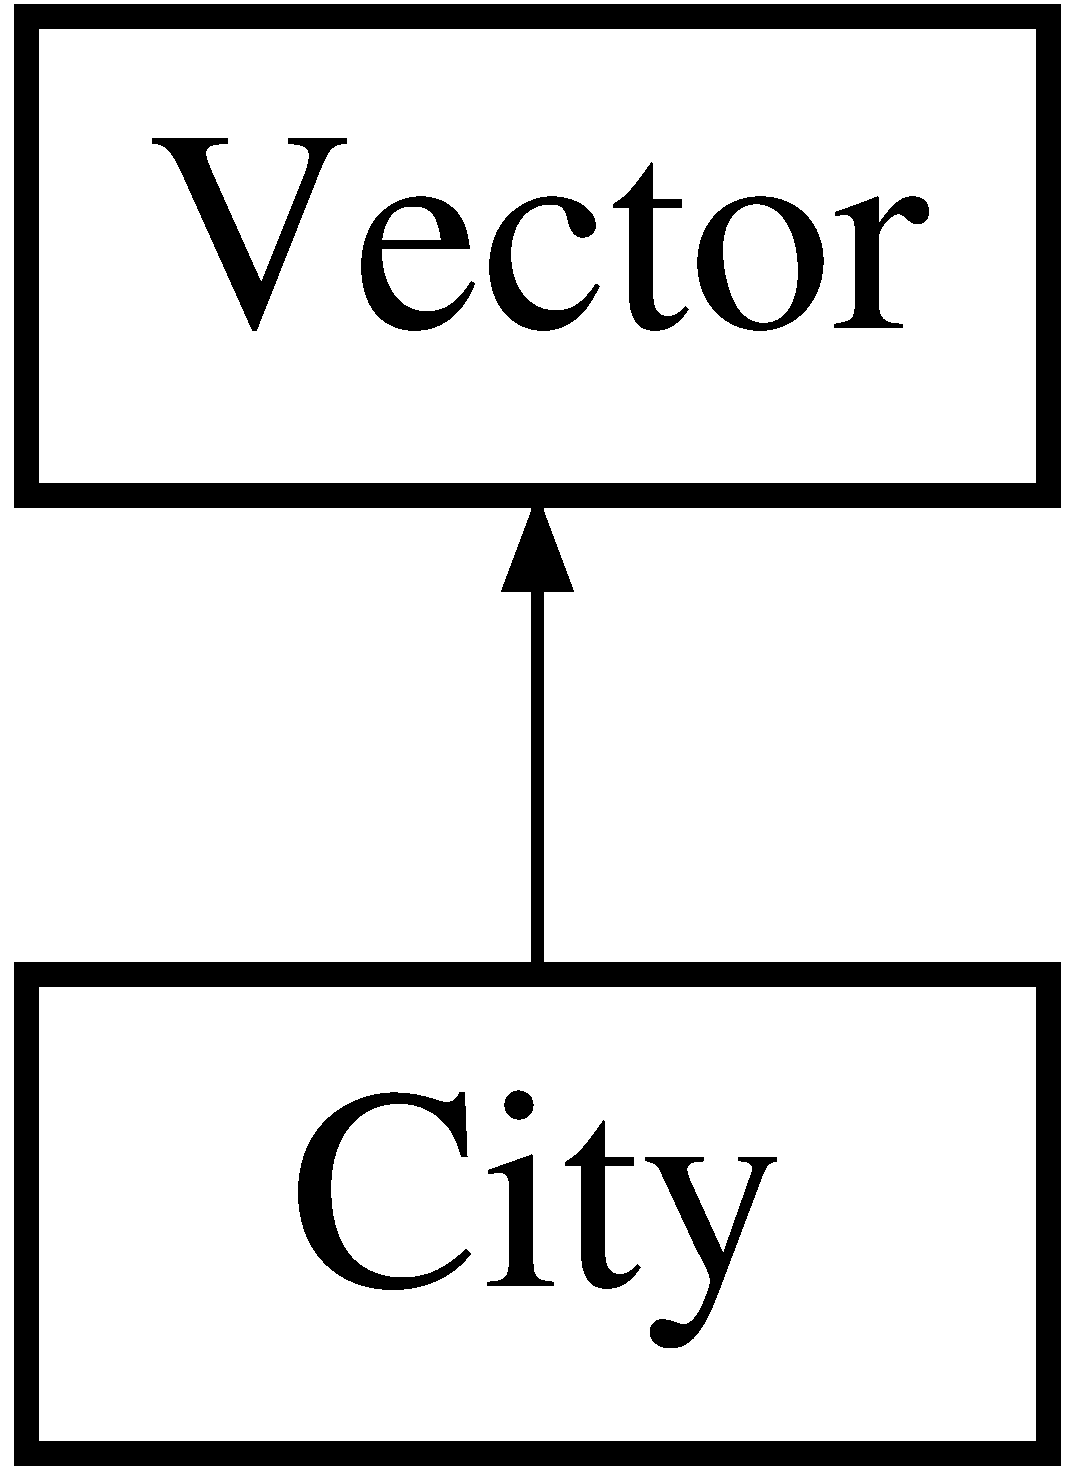
\includegraphics[height=2.000000cm]{class_city}
\end{center}
\end{figure}
\subsection*{Public Member Functions}
\begin{DoxyCompactItemize}
\item 
{\bfseries City} (string name, C\-I\-T\-Y\-C\-O\-L\-O\-U\-R city\-Colour, short number, {\bf Vector} place)\label{class_city_a086f1d9fd30ad0bcedcf72d526cbf365}

\end{DoxyCompactItemize}
\subsection*{Public Attributes}
\begin{DoxyCompactItemize}
\item 
string {\bfseries name}\label{class_city_a38b5e8b9bd4e263434eae0344913d341}

\item 
C\-I\-T\-Y\-C\-O\-L\-O\-U\-R {\bfseries city\-Colour}\label{class_city_a49ce7573be0c500755ffc346399a7ae3}

\item 
short {\bfseries number}\label{class_city_a0fecf97dc1cbd61bb1bd27325decad52}

\end{DoxyCompactItemize}


The documentation for this class was generated from the following files\-:\begin{DoxyCompactItemize}
\item 
hdr/game/City.\-h\item 
src/game/City.\-cpp\end{DoxyCompactItemize}

\section{Connection Class Reference}
\label{class_connection}\index{Connection@{Connection}}
\subsection*{Public Member Functions}
\begin{DoxyCompactItemize}
\item 
{\bfseries Connection} (const {\bf Coordinate} \&erste, const {\bf Coordinate} \&zweite, bool Hindernis)\label{class_connection_acff2b5b881817a7b6e8d8173a1937640}

\item 
const {\bf Connection} \& {\bfseries operator=} (const {\bf Connection} \&) const \label{class_connection_a715ee5805776e50b971d5772267e4b46}

\item 
void {\bfseries dump} () const \label{class_connection_a67b9ea26a5f1419c2715e87f26dbb2f4}

\end{DoxyCompactItemize}
\subsection*{Public Attributes}
\begin{DoxyCompactItemize}
\item 
const {\bf Coordinate} \& {\bfseries first}\label{class_connection_a1e4300e2849a2daebf4b1e4577ef1ea8}

\item 
const {\bf Coordinate} \& {\bfseries second}\label{class_connection_a968eaf3cec0996491425d8569e42416f}

\item 
const D\-I\-R\-E\-C\-T\-I\-O\-N {\bfseries direction}\label{class_connection_aa417c011125675e3faf7f5ec1fe4192b}

\item 
const bool {\bfseries hindernis}\label{class_connection_ae29f9a099c5d00919eb45123864fb7f4}

\end{DoxyCompactItemize}


The documentation for this class was generated from the following files\-:\begin{DoxyCompactItemize}
\item 
hdr/game/Connection.\-h\item 
src/game/Connection.\-cpp\end{DoxyCompactItemize}

\hypertarget{class_coordinate}{\section{Coordinate Class Reference}
\label{class_coordinate}\index{Coordinate@{Coordinate}}
}


{\ttfamily \#include $<$Koordinate.\-h$>$}

Inheritance diagram for Coordinate\-:\begin{figure}[H]
\begin{center}
\leavevmode
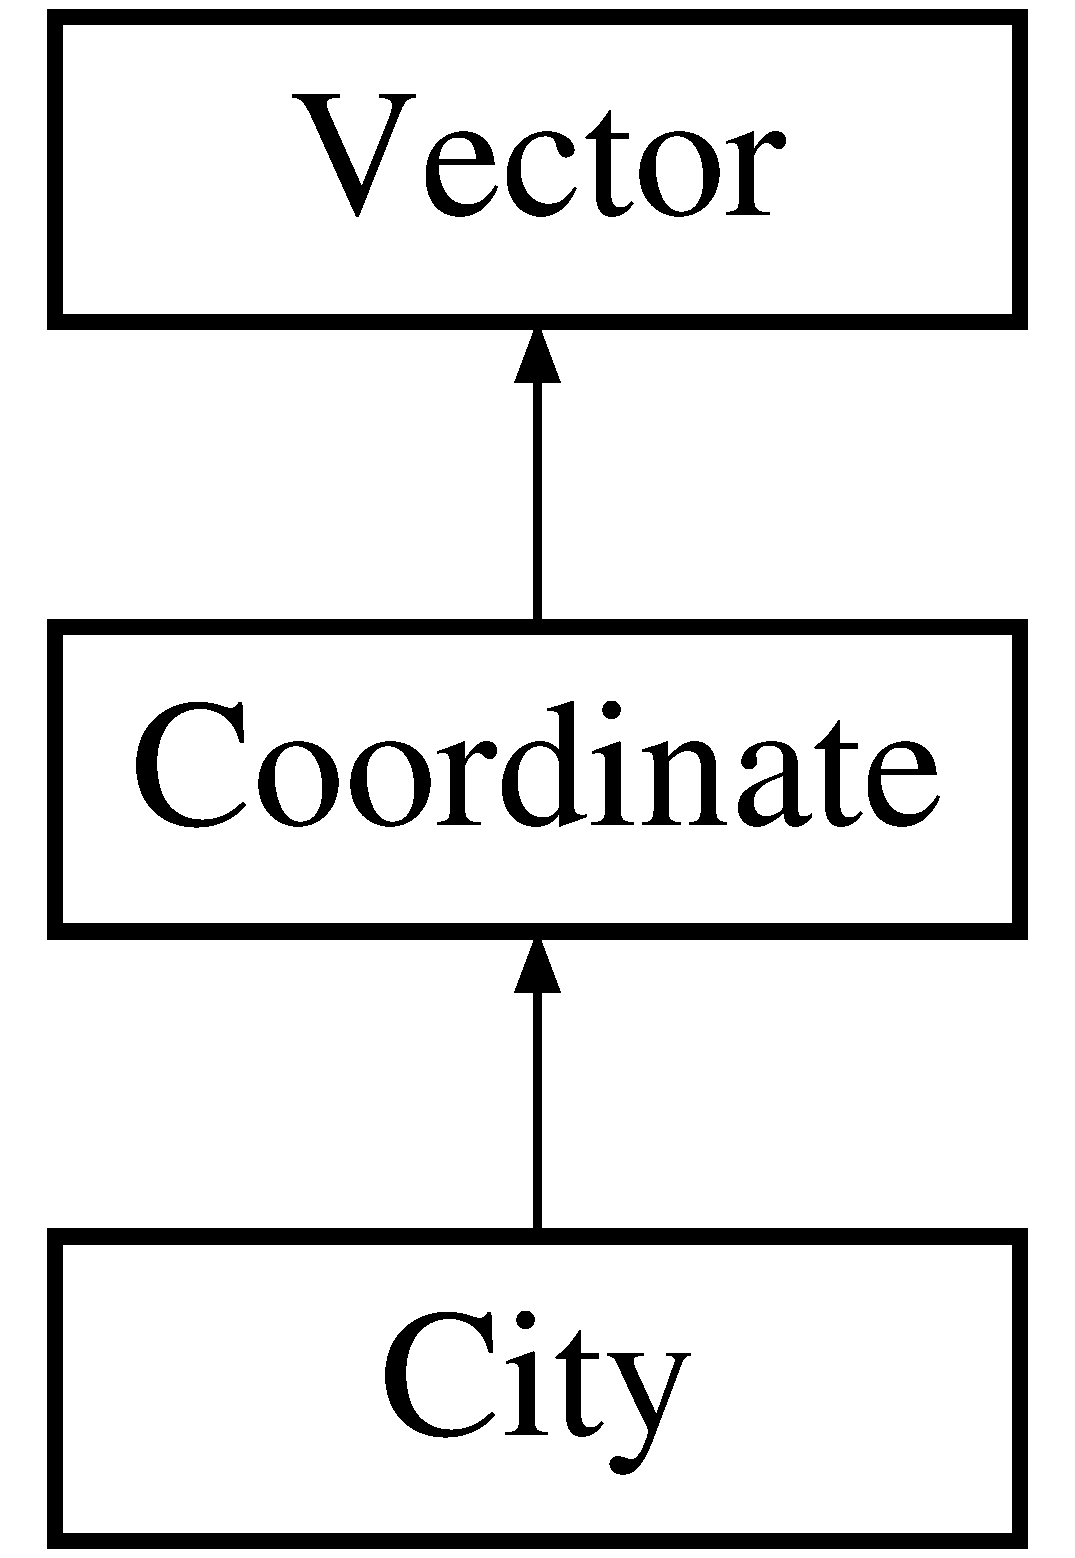
\includegraphics[height=2.000000cm]{class_coordinate}
\end{center}
\end{figure}
\subsection*{Public Member Functions}
\begin{DoxyCompactItemize}
\item 
\hypertarget{class_coordinate_afa539ca7218f25717e25482babf0bfc9}{{\bfseries Coordinate} (short x, short y)}\label{class_coordinate_afa539ca7218f25717e25482babf0bfc9}

\item 
\hypertarget{class_coordinate_a6f212c6c04f0f87e09157cff2092c111}{{\bfseries Coordinate} (short x, short y, const \hyperlink{class_city}{City} \&City\-On\-Coordinate)}\label{class_coordinate_a6f212c6c04f0f87e09157cff2092c111}

\end{DoxyCompactItemize}
\subsection*{Public Attributes}
\begin{DoxyCompactItemize}
\item 
\hypertarget{class_coordinate_a68372ad69c745041d63625c2a9ed4577}{const \hyperlink{class_city}{City} \& {\bfseries vor\-Ort}}\label{class_coordinate_a68372ad69c745041d63625c2a9ed4577}

\item 
\hypertarget{class_coordinate_ac7c3032bcd943e1e0d3576d6ec39745a}{bool {\bfseries Null}}\label{class_coordinate_ac7c3032bcd943e1e0d3576d6ec39745a}

\end{DoxyCompactItemize}


\subsection{Detailed Description}
Objects of this class are coordiantes on the board, where the x-\/axis is parallel to the west-\/east direction and the y-\/axis parallel to the north-\/(south-\/west) direction. The (0,0) coordinate is the most upper left corner of the board. The range of the x-\/values is from 0 to M\-A\-X\-\_\-\-X and the y-\/values from 0 to M\-A\-X\-\_\-\-Y. 

The documentation for this class was generated from the following files\-:\begin{DoxyCompactItemize}
\item 
Koordinate.\-h\item 
Koordinate.\-cpp\end{DoxyCompactItemize}

\section{Counter Class Reference}
\label{class_counter}\index{Counter@{Counter}}
\subsection*{Public Member Functions}
\begin{DoxyCompactItemize}
\item 
{\bfseries Counter} (const {\bf Counter} \&copy)\label{class_counter_ae36386566b1cc1bfbce065dd182e1e1e}

\item 
int {\bfseries add} ({\bf A\-I} $\ast$player, int counter)\label{class_counter_a7f4afd6b55161dee82b1e046af77924b}

\item 
int {\bfseries get} ({\bf A\-I} $\ast$player) const \label{class_counter_a95c8f10bc296a35599cb97f3dc33f0e9}

\item 
{\bf Counter} {\bfseries operator+} (const {\bf Counter} \&rhs) const \label{class_counter_af13b8092fbef704e68fdefb2d024683a}

\item 
{\bf Counter} {\bfseries operator-\/} (const {\bf Counter} \&rhs) const \label{class_counter_a563604893f4bc66449ac9901928ebbc4}

\item 
{\bf Counter} {\bfseries operator=} (const {\bf Counter} \&copy)\label{class_counter_a683fff5c5b2fb7082f637a817106ec4f}

\item 
{\bf Counter} {\bfseries operator+=} (const {\bf Counter} \&rhs)\label{class_counter_a0923b8779d18168542db7281bdb7c6c2}

\item 
{\bf Counter} {\bfseries operator-\/=} (const {\bf Counter} \&rhs)\label{class_counter_a99857e9ec0584d6525fc49e00223b555}

\end{DoxyCompactItemize}


The documentation for this class was generated from the following files\-:\begin{DoxyCompactItemize}
\item 
hdr/game/Counter.\-h\item 
src/game/Counter.\-cpp\end{DoxyCompactItemize}

\section{Game Class Reference}
\label{class_game}\index{Game@{Game}}
\subsection*{Public Member Functions}
\begin{DoxyCompactItemize}
\item 
{\bfseries Game} ({\bf Game\-Logger} $\ast$game\-Logger)\label{class_game_a9f03a276b1af77e70e794ac22ded922e}

\item 
void {\bfseries play} ()\label{class_game_aa333825d0bca80e91e53c7e23f053405}

\end{DoxyCompactItemize}


The documentation for this class was generated from the following files\-:\begin{DoxyCompactItemize}
\item 
hdr/game/Game.\-h\item 
src/game/Game.\-cpp\end{DoxyCompactItemize}

\section{Game\-Logger Class Reference}
\label{class_game_logger}\index{Game\-Logger@{Game\-Logger}}
\subsection*{Public Member Functions}
\begin{DoxyCompactItemize}
\item 
{\bfseries Game\-Logger} (const {\bf Simulation\-Logger} $\ast$simulation\-Logger, const {\bf Playing\-Order} playing\-Order, const {\bf A\-I} $\ast$game\-Starting\-Player)\label{class_game_logger_a9ccd538027b996730e546a936bfd97ea}

\item 
const {\bf Board} \& {\bfseries get\-Board} () const \label{class_game_logger_a200f1e95042330a8568a8c1e1d679529}

\item 
int {\bfseries get\-Dead\-Line} () const \label{class_game_logger_ad5181081324043367b7b3c04c461182d}

\item 
const {\bf A\-I} $\ast$ {\bfseries get\-Game\-Starting\-Player} () const \label{class_game_logger_a9d8059f296f6a4eb836c21059d82b468}

\item 
const vector$<$ {\bf A\-I} $\ast$ $>$ \& {\bfseries get\-Player\-List} () const \label{class_game_logger_a304f93438a2c2edded594de4e2a1d421}

\item 
const {\bf Playing\-Order} \& {\bfseries get\-Playing\-Order} () const \label{class_game_logger_a66bf007670b3934bee8e5538d7388001}

\item 
const {\bf Counter} \& {\bfseries get\-Points} () const \label{class_game_logger_a987619dec293b5ec4add94f41ab6f733}

\item 
const vector$<$ {\bf Round\-Logger} $\ast$ $>$ \& {\bfseries get\-Round\-List} () const \label{class_game_logger_a7c79f75b48e6a1e9f924f44408ae752f}

\item 
const {\bf Counter} \& {\bfseries get\-Game\-Won} () const \label{class_game_logger_ad499b496c00c5f25a484a90afd533c66}

\end{DoxyCompactItemize}
\subsection*{Friends}
\begin{DoxyCompactItemize}
\item 
class {\bfseries Game}\label{class_game_logger_aa2fab026580d6f14280c2ffb8063a314}

\end{DoxyCompactItemize}


The documentation for this class was generated from the following files\-:\begin{DoxyCompactItemize}
\item 
hdr/logger/Game\-Logger.\-h\item 
src/logger/Game\-Logger.\-cpp\end{DoxyCompactItemize}

\section{Human Class Reference}
\label{class_human}\index{Human@{Human}}
Inheritance diagram for Human\-:\begin{figure}[H]
\begin{center}
\leavevmode
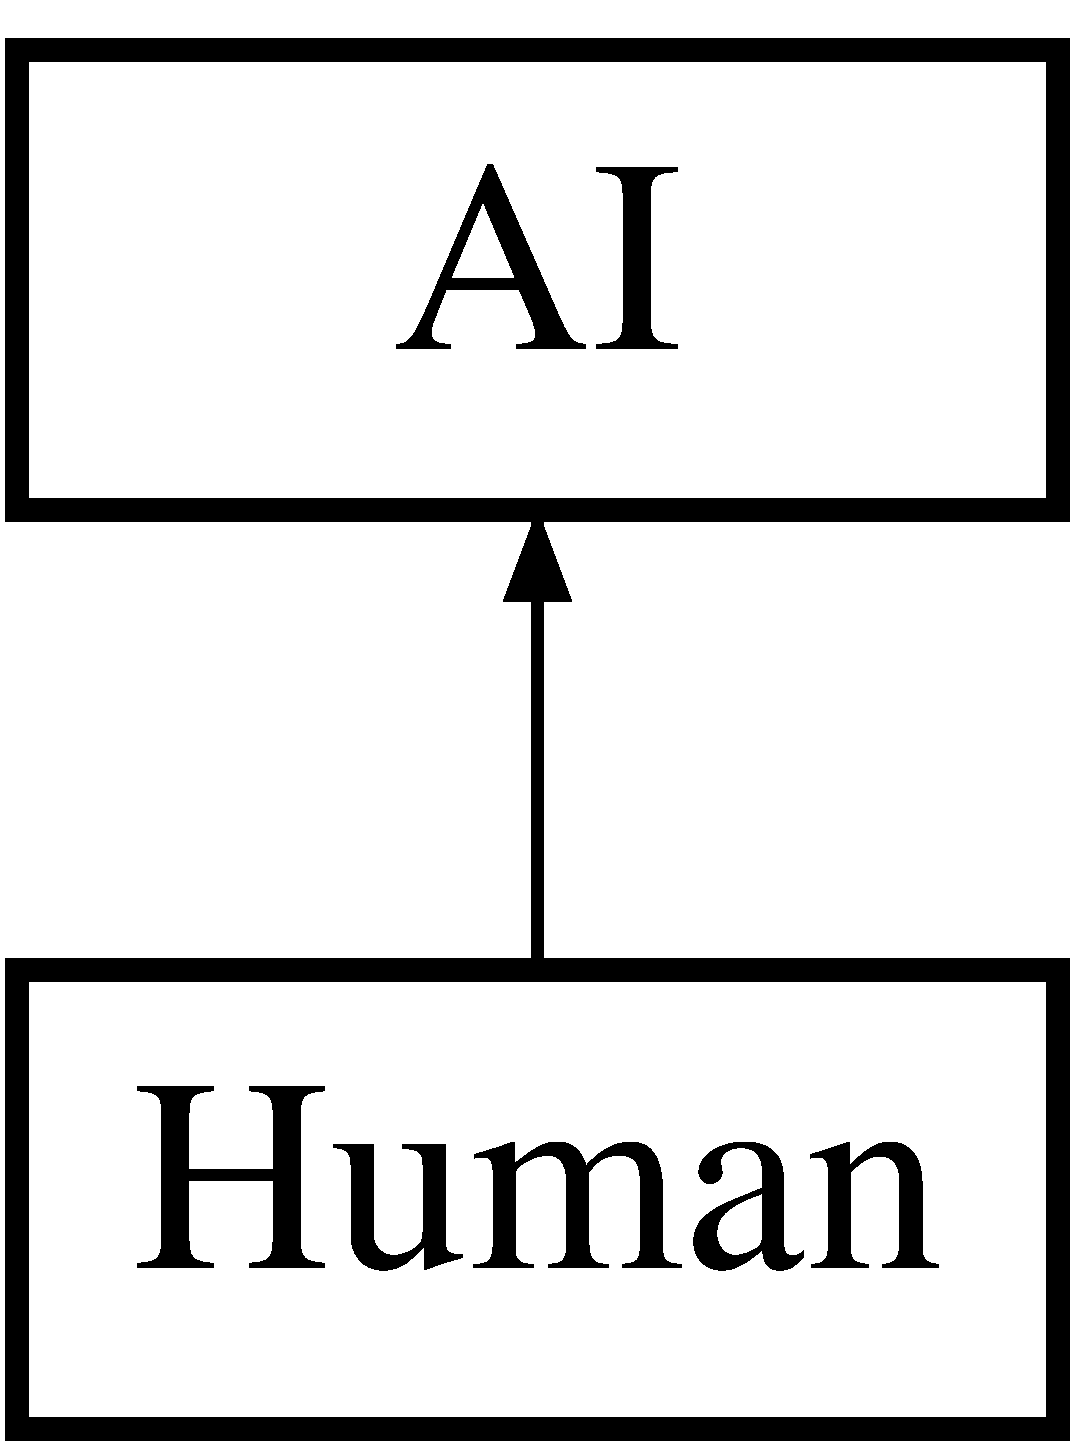
\includegraphics[height=2.000000cm]{class_human}
\end{center}
\end{figure}
\subsection*{Public Member Functions}
\begin{DoxyCompactItemize}
\item 
{\bfseries Human} (P\-L\-A\-Y\-E\-R\-C\-O\-L\-O\-R {\bf player\-Color}, {\bf User\-Input\-Window} $\ast$uiexec)\label{class_human_aad9ae63105013786063e50144a46e3db}

\item 
{\bf Move} {\bf do\-Move} ({\bf State} \&, vector$<$ {\bf Move} $\ast$ $>$)
\item 
{\bf Vector} {\bf set\-Pawn} ({\bf State} \&)
\item 
bool {\bfseries count\-Points} ({\bf State} \&, vector$<$ {\bf Connection} $\ast$ $>$)\label{class_human_a97378e4328a84ce3b0b0e7695bcdd432}

\item 
void {\bf gather\-Information\-End\-Of\-Round} (const {\bf Round\-Logger} $\ast$)
\end{DoxyCompactItemize}
\subsection*{Additional Inherited Members}


\subsection{Member Function Documentation}
\index{Human@{Human}!do\-Move@{do\-Move}}
\index{do\-Move@{do\-Move}!Human@{Human}}
\subsubsection[{do\-Move}]{\setlength{\rightskip}{0pt plus 5cm}{\bf Move} Human\-::do\-Move (
\begin{DoxyParamCaption}
\item[{{\bf State} \&}]{aktuell, }
\item[{vector$<$ {\bf Move} $\ast$ $>$}]{move\-List}
\end{DoxyParamCaption}
)\hspace{0.3cm}{\ttfamily [virtual]}}\label{class_human_a797f11c25934d3e6ebdfa612715f899a}
Inside this methode you calculate your next move in the game. 

Implements {\bf A\-I} \doxyref{}{p.}{class_a_i_ade352ac8d216d67feca731a127b50e6f}.

\index{Human@{Human}!gather\-Information\-End\-Of\-Round@{gather\-Information\-End\-Of\-Round}}
\index{gather\-Information\-End\-Of\-Round@{gather\-Information\-End\-Of\-Round}!Human@{Human}}
\subsubsection[{gather\-Information\-End\-Of\-Round}]{\setlength{\rightskip}{0pt plus 5cm}void Human\-::gather\-Information\-End\-Of\-Round (
\begin{DoxyParamCaption}
\item[{const {\bf Round\-Logger} $\ast$}]{current\-Infos}
\end{DoxyParamCaption}
)\hspace{0.3cm}{\ttfamily [virtual]}}\label{class_human_af9bb973f12694c98e504766193a4652f}
At the end of each round you can take a look at the whole game and the playing cards of your opponents. This can be usefull, if you want to figure out there strategy and react to that over a simulation period. 

Implements {\bf A\-I} \doxyref{}{p.}{class_a_i_a8565a9ef04ac4f9913913c99f65213b2}.

\index{Human@{Human}!set\-Pawn@{set\-Pawn}}
\index{set\-Pawn@{set\-Pawn}!Human@{Human}}
\subsubsection[{set\-Pawn}]{\setlength{\rightskip}{0pt plus 5cm}{\bf Vector} Human\-::set\-Pawn (
\begin{DoxyParamCaption}
\item[{{\bf State} \&}]{aktuell}
\end{DoxyParamCaption}
)\hspace{0.3cm}{\ttfamily [virtual]}}\label{class_human_a31b9983eba5b8ccd37c7b41b4ecba912}
At the beginning of each round you have to define your starting position of your pawn. 

Implements {\bf A\-I} \doxyref{}{p.}{class_a_i_a0fbc5b7d4230575baf80217d0c250cc9}.



The documentation for this class was generated from the following files\-:\begin{DoxyCompactItemize}
\item 
hdr/game/Human.\-h\item 
src/game/Human.\-cpp\end{DoxyCompactItemize}

\section{Playing\-Order\-:\-:iterator Class Reference}
\label{class_playing_order_1_1iterator}\index{Playing\-Order\-::iterator@{Playing\-Order\-::iterator}}
\subsection*{Public Member Functions}
\begin{DoxyCompactItemize}
\item 
{\bfseries iterator} (Playing\-Order\-Element $\ast$cursor)\label{class_playing_order_1_1iterator_aa1acaaf5aa4cb04b45d688bdb2585cb7}

\item 
{\bf A\-I} $\ast$ {\bfseries operator-\/$>$} () const \label{class_playing_order_1_1iterator_ae273376a2c7a09cbad0ddc17a9120a57}

\item 
{\bf A\-I} $\ast$ {\bfseries operator$\ast$} () const \label{class_playing_order_1_1iterator_a766bf56248a6beb3a7515de7fe6e85f0}

\item 
{\bf iterator} {\bfseries operator++} ()\label{class_playing_order_1_1iterator_a53d94a59d257d705067a6631c11b31cc}

\item 
bool {\bfseries operator!=} (const {\bf Playing\-Order\-::iterator} \&rhs) const \label{class_playing_order_1_1iterator_aff6e658fd7eb13f7538bcd88efd66ad2}

\end{DoxyCompactItemize}
\subsection*{Public Attributes}
\begin{DoxyCompactItemize}
\item 
Playing\-Order\-Element $\ast$ {\bfseries cursor}\label{class_playing_order_1_1iterator_a8685cc1ee395f5b45ea6ec85c2110ebd}

\end{DoxyCompactItemize}


The documentation for this class was generated from the following files\-:\begin{DoxyCompactItemize}
\item 
game/header/Playing\-Order.\-h\item 
game/source/iterator.\-cpp\end{DoxyCompactItemize}

\hypertarget{class_move}{\section{Move Class Reference}
\label{class_move}\index{Move@{Move}}
}
\subsection*{Public Member Functions}
\begin{DoxyCompactItemize}
\item 
\hypertarget{class_move_adad54af2a6af52e8a1b37cc0c28a9c03}{{\bfseries Move} (short spielerfarbe, const \hyperlink{class_verbindung}{Verbindung} $\ast$belegt1, const \hyperlink{class_verbindung}{Verbindung} $\ast$belegt2)}\label{class_move_adad54af2a6af52e8a1b37cc0c28a9c03}

\item 
\hypertarget{class_move_a4a681053577ea9b245e8794c427fe910}{bool {\bfseries gueltig} (\hyperlink{class_zustand}{Zustand}, short)}\label{class_move_a4a681053577ea9b245e8794c427fe910}

\item 
\hypertarget{class_move_a982e038b4f43336bf8396d8e63f9cebb}{void {\bfseries ausfuehren} (\hyperlink{class_zustand}{Zustand} \&) const }\label{class_move_a982e038b4f43336bf8396d8e63f9cebb}

\item 
\hypertarget{class_move_a5fd65957977d9e30fd8898fa4a14ac56}{void {\bfseries dump} () const }\label{class_move_a5fd65957977d9e30fd8898fa4a14ac56}

\item 
\hypertarget{class_move_a2cae41881447ddc9496cff2800ce01e2}{\hyperlink{class_move}{Move} \& {\bfseries operator=} (const \hyperlink{class_move}{Move} \&zuweisung)}\label{class_move_a2cae41881447ddc9496cff2800ce01e2}

\end{DoxyCompactItemize}


The documentation for this class was generated from the following files\-:\begin{DoxyCompactItemize}
\item 
Move.\-h\item 
Move.\-cpp\end{DoxyCompactItemize}

\section{Pawn Class Reference}
\label{class_pawn}\index{Pawn@{Pawn}}
Inheritance diagram for Pawn\-:\begin{figure}[H]
\begin{center}
\leavevmode
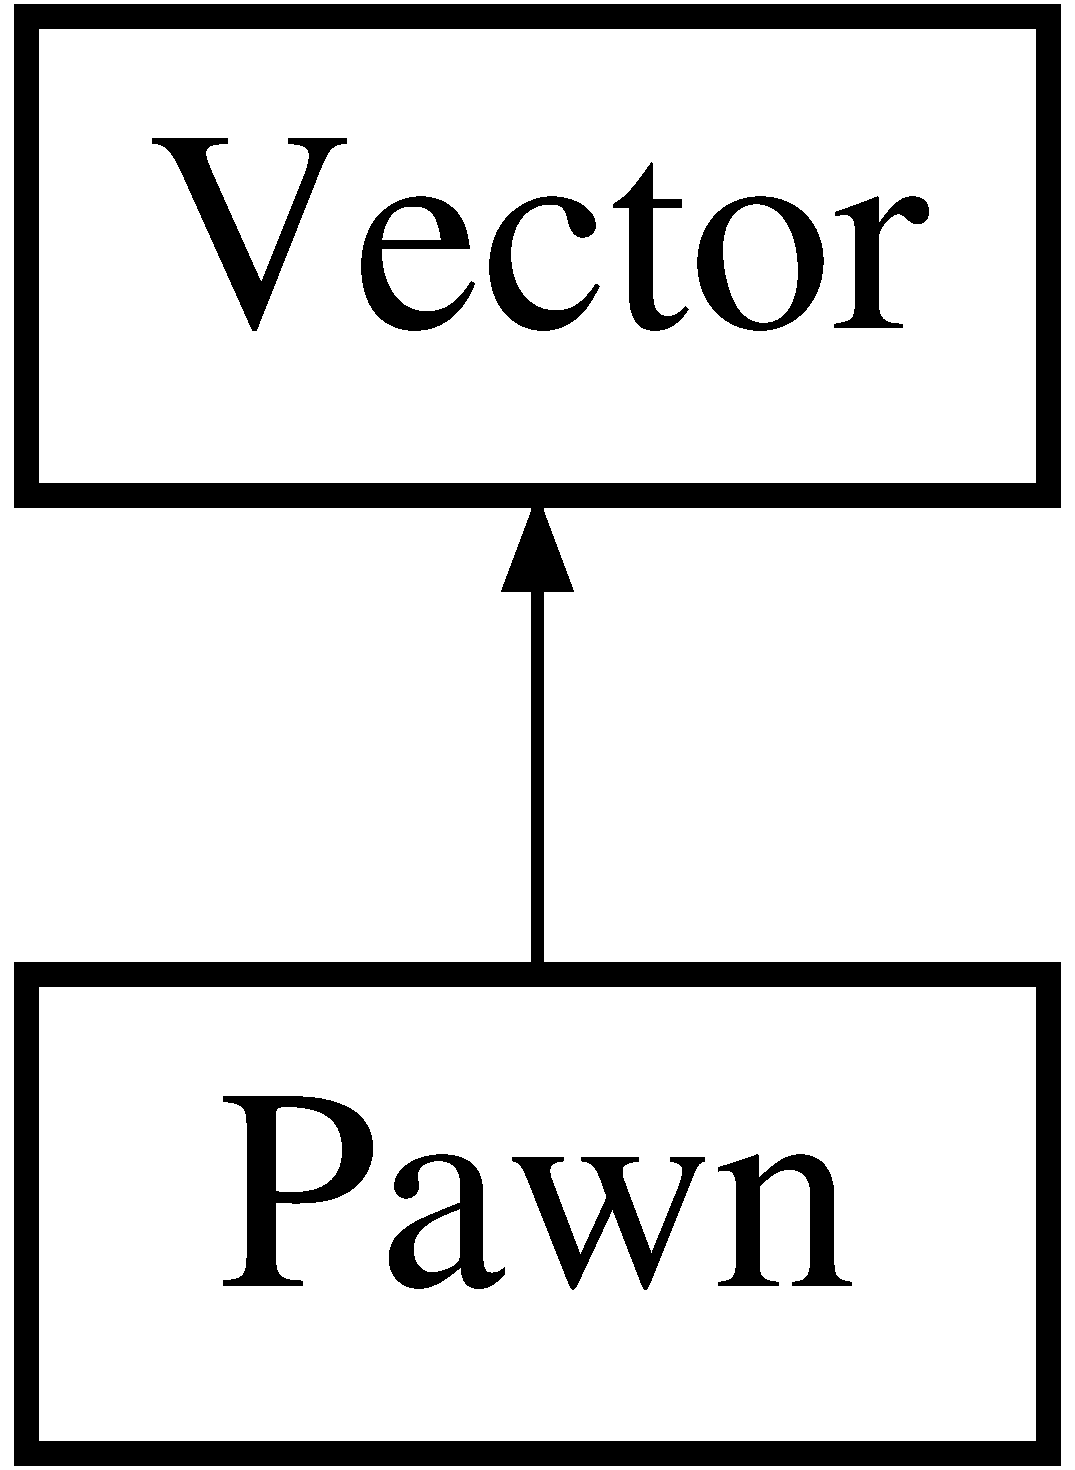
\includegraphics[height=2.000000cm]{class_pawn}
\end{center}
\end{figure}
\subsection*{Public Member Functions}
\begin{DoxyCompactItemize}
\item 
{\bfseries Pawn} (P\-L\-A\-Y\-E\-R\-C\-O\-L\-O\-U\-R colour, {\bf Vector} pos)\label{class_pawn_a0b393cf205a91f3ac07bdfbc14036fe2}

\item 
{\bfseries Pawn} (const {\bf Pawn} \&copy)\label{class_pawn_a512724e66a28f71702973bcd87bd883b}

\end{DoxyCompactItemize}
\subsection*{Public Attributes}
\begin{DoxyCompactItemize}
\item 
short {\bfseries schienennetznummer}\label{class_pawn_a8f02932d671c756305cbe3959104d5bf}

\item 
const P\-L\-A\-Y\-E\-R\-C\-O\-L\-O\-U\-R {\bfseries spielerfarbe}\label{class_pawn_afa1487b79a518e686b8334ae6467ae55}

\end{DoxyCompactItemize}


The documentation for this class was generated from the following files\-:\begin{DoxyCompactItemize}
\item 
game/header/Pawn.\-h\item 
game/source/Pawn.\-cpp\end{DoxyCompactItemize}

\section{Playing\-Order Class Reference}
\label{class_playing_order}\index{Playing\-Order@{Playing\-Order}}
\subsection*{Classes}
\begin{DoxyCompactItemize}
\item 
class {\bf iterator}
\end{DoxyCompactItemize}
\subsection*{Public Member Functions}
\begin{DoxyCompactItemize}
\item 
{\bfseries Playing\-Order} (std\-::vector$<$ {\bf A\-I} $\ast$ $>$ order)\label{class_playing_order_a7f530887195bc39170e48628fe33a2e8}

\item 
{\bf Playing\-Order\-::iterator} {\bfseries begin} ({\bf A\-I} $\ast$player) const \label{class_playing_order_ae84e1df8d1e7cbce8787895375a1a1f2}

\end{DoxyCompactItemize}


The documentation for this class was generated from the following files\-:\begin{DoxyCompactItemize}
\item 
hdr/game/Playing\-Order.\-h\item 
src/game/Playing\-Order.\-cpp\end{DoxyCompactItemize}

\section{Round Class Reference}
\label{class_round}\index{Round@{Round}}
\subsection*{Public Member Functions}
\begin{DoxyCompactItemize}
\item 
{\bfseries Round} ({\bf Round\-Logger} $\ast$round\-Logger)\label{class_round_abbe52774d5d8aa3821fb98da60cfbb2c}

\item 
void {\bfseries play} ()\label{class_round_a5f82d0ce31d620c9e649fb5b565c79b4}

\end{DoxyCompactItemize}
\subsection*{Public Attributes}
\begin{DoxyCompactItemize}
\item 
{\bf State} {\bfseries current\-State}\label{class_round_ae453f02f4bf081afa39f79779cbb6577}

\end{DoxyCompactItemize}


The documentation for this class was generated from the following files\-:\begin{DoxyCompactItemize}
\item 
game/header/Round.\-h\item 
game/source/Round.\-cpp\end{DoxyCompactItemize}

\section{Round\-Logger Class Reference}
\label{class_round_logger}\index{Round\-Logger@{Round\-Logger}}
\subsection*{Public Member Functions}
\begin{DoxyCompactItemize}
\item 
{\bfseries Round\-Logger} ({\bf Playing\-Order} \&playing\-Order, std\-::vector$<$ {\bf A\-I} $\ast$ $>$ player\-List, {\bf Board} \&board, {\bf A\-I} $\ast$round\-Starting\-Player)\label{class_round_logger_a319ff2d7dee4b15c102138bda1b027fc}

\end{DoxyCompactItemize}
\subsection*{Public Attributes}
\begin{DoxyCompactItemize}
\item 
{\bf Playing\-Order} \& {\bfseries playing\-Order}\label{class_round_logger_a7fd0f9fd826753aa3715ba85e863ab3f}

\item 
std\-::vector$<$ {\bf A\-I} $\ast$ $>$ {\bfseries player\-List}\label{class_round_logger_aebd799e774b85f36a77e1fa4cfe5687b}

\item 
{\bf Board} \& {\bfseries board}\label{class_round_logger_a256a2d63cc85c71f8a57268b1829e6df}

\item 
{\bf A\-I} $\ast$ {\bfseries round\-Starting\-Player}\label{class_round_logger_adfb669d859b3e9e1bd18a8ae1a31cf6b}

\item 
{\bf City} $\ast$$\ast$ {\bfseries playing\-Cards}\label{class_round_logger_a4e30b0c6cf75d64dd8c3af86e240e188}

\item 
{\bf Counter} {\bfseries lost\-Points}\label{class_round_logger_a48257ec06504aa78fc89fe943d06aca8}

\item 
{\bf Pawn} $\ast$$\ast$ {\bfseries pawn\-List}\label{class_round_logger_a3ba92d778f19c90572cfa6d7df0dcd5f}

\item 
std\-::vector$<$ {\bf Move} $\ast$ $>$ {\bfseries move\-List}\label{class_round_logger_a0c998b04cc3185ea20d2a7444cda1323}

\end{DoxyCompactItemize}


The documentation for this class was generated from the following files\-:\begin{DoxyCompactItemize}
\item 
logger/header/Round\-Logger.\-h\item 
logger/source/Round\-Logger.\-cpp\end{DoxyCompactItemize}

\section{Simulation Class Reference}
\label{class_simulation}\index{Simulation@{Simulation}}
\subsection*{Public Member Functions}
\begin{DoxyCompactItemize}
\item 
{\bfseries Simulation} ({\bf Simulation\-Logger} $\ast$simulation\-Logger)\label{class_simulation_ac7a66a0b7cca01eaf41e4a1c922ffa42}

\item 
void {\bfseries run} ()\label{class_simulation_ae5c367f87c0b5dc9740bc6d00e44e72c}

\end{DoxyCompactItemize}


The documentation for this class was generated from the following files\-:\begin{DoxyCompactItemize}
\item 
hdr/game/Simulation.\-h\item 
src/game/Simulation.\-cpp\end{DoxyCompactItemize}

\section{Simulation\-Logger Class Reference}
\label{class_simulation_logger}\index{Simulation\-Logger@{Simulation\-Logger}}
\subsection*{Public Member Functions}
\begin{DoxyCompactItemize}
\item 
{\bfseries Simulation\-Logger} (std\-::vector$<$ {\bf A\-I} $\ast$ $>$ player\-List, {\bf Board} \&board, int number\-Of\-Players, unsigned int seed=(unsigned) time(0))\label{class_simulation_logger_a37a43872a7fbee07130e3b39460b54c6}

\item 
std\-::vector$<$ {\bf A\-I} $\ast$ $>$ {\bfseries get\-Playing\-Order} (int simulation\-Number)\label{class_simulation_logger_a4ff55e48a33b19bbd8108d33c9ccf2bf}

\end{DoxyCompactItemize}
\subsection*{Public Attributes}
\begin{DoxyCompactItemize}
\item 
std\-::vector$<$ {\bf A\-I} $\ast$ $>$ {\bfseries player\-List}\label{class_simulation_logger_a344898f3a4cd7df47e8e7dafd0ff5bd6}

\item 
{\bf Counter} {\bfseries games\-Won}\label{class_simulation_logger_ab3ee79eb79f0c07d42ebebebf057587b}

\item 
std\-::vector$<$ {\bf Game\-Logger} $\ast$ $>$ {\bfseries game\-List}\label{class_simulation_logger_abe55e6d0fb8933d3f7f289a1f255f1ad}

\item 
{\bf Board} {\bfseries board}\label{class_simulation_logger_a224021a57c2a155d5bec0548d6368fe1}

\item 
unsigned int {\bfseries seed}\label{class_simulation_logger_a9af9361d2d81c2e0fd47a5fb26285761}

\end{DoxyCompactItemize}


The documentation for this class was generated from the following files\-:\begin{DoxyCompactItemize}
\item 
hdr/logger/Simulation\-Logger.\-h\item 
src/logger/Simulation\-Logger.\-cpp\end{DoxyCompactItemize}

\section{State Class Reference}
\label{class_state}\index{State@{State}}
\subsection*{Public Member Functions}
\begin{DoxyCompactItemize}
\item 
{\bfseries State} ({\bf Board} \&{\bf Spielbrett})\label{class_state_ab8e8b562af12bba2ae71a14fcfd87673}

\item 
{\bfseries State} (const {\bf State} \&)\label{class_state_a5ca97340266d486dfa42225f19c40de3}

\item 
{\bf Pawn} {\bfseries get\-Poeppel} (const P\-L\-A\-Y\-E\-R\-C\-O\-L\-O\-U\-R spielerfarbe) const \label{class_state_a5ddfbac7a481236179ace80166f69da8}

\item 
bool {\bfseries schienen\-Netz\-Nummer\-Von\-\_\-\-Ist\-\_\-} (const {\bf Connection} \&, const short schienennr) const \label{class_state_a974ccf0cdff0adc321603f11c8df7970}

\item 
short {\bfseries get\-Schienen\-Netz\-Nummer} (const {\bf Vector} \&koo) const \label{class_state_a5d32c5f1439d14757830b7bbd6fde7cb}

\item 
void {\bfseries set\-Schienen\-Netz\-Nummer} (const {\bf Coordinate} \&koo, const short nr)\label{class_state_a61e844e517116c5ec1eaeb6886906df8}

\item 
void {\bfseries set\-Schiene} (const {\bf Connection} \&)\label{class_state_afa0cf80f1e1cc065fd63372c8ffc19be}

\item 
void {\bfseries reset\-Nr\-\_\-\-Zu\-Nr\-\_\-} (const short, const short)\label{class_state_ade757a61a90c393f8b7a3495221f1779}

\item 
void {\bfseries schiene\-Legen} (const {\bf Connection} \&)\label{class_state_a76034aee14f5704a970a7b4a831935e7}

\item 
const {\bf Connection} $\ast$ {\bfseries get\-Verbindung} ({\bf Vector} a, {\bf Vector} b) const \label{class_state_a668add718e776deb4fd34c5dbaeabfb5}

\item 
void {\bfseries add\-Pawn} ({\bf Pawn} insert)\label{class_state_a9a192466fc65d42a405b6c461f5ae1c7}

\item 
void {\bfseries reset\-All} ()\label{class_state_ae3cf3d6f8fd90d8a59d53ccb1290a46c}

\item 
unsigned short $\ast$$\ast$ {\bfseries evaluate\-Board} ({\bf Vector} target) const \label{class_state_a5bc0dd359e67c72d457a64277afaf621}

\item 
unsigned short {\bfseries distance} ({\bf Vector} target, const vector$<$ {\bf Vector} $>$ \&possible\-Starts) const \label{class_state_a2e17c63ec7373cf144f37933bef1d197}

\item 
vector$<$ {\bf Vector} $>$ {\bfseries points\-Belonging\-To\-Railway\-System} (P\-L\-A\-Y\-E\-R\-C\-O\-L\-O\-U\-R playercolour) const \label{class_state_ab039ad1b0cb7721e26946c79faff16d5}

\item 
void {\bfseries akt\-Ausgabe} () const \label{class_state_ade0adf3c0871edde2df2370718f0c8f6}

\item 
void {\bfseries set\-Round} (short x)\label{class_state_a468eb35199b879f9df58245540ca849c}

\item 
void {\bfseries set\-Turn} (short x)\label{class_state_a5f8cd95cb039eb5333a9fed80b7efd2f}

\item 
void {\bfseries set\-Players\-Turn} (P\-L\-A\-Y\-E\-R\-C\-O\-L\-O\-U\-R x)\label{class_state_af71c2a4c5a5c3969d3a6ac61e4d4e6d4}

\end{DoxyCompactItemize}
\subsection*{Static Public Member Functions}
\begin{DoxyCompactItemize}
\item 
static short {\bfseries Richtungs\-Wert} (const {\bf Vector} \&)\label{class_state_ac1f87995c4da93c0a24f0d5564b8644c}

\end{DoxyCompactItemize}
\subsection*{Public Attributes}
\begin{DoxyCompactItemize}
\item 
short $\ast$$\ast$ {\bfseries schienen\-Netz\-Nummer}\label{class_state_aa596bf79a270efaacec2cdcc523c29cb}

\item 
bool $\ast$$\ast$$\ast$ {\bfseries schiene\-Gelegt}\label{class_state_a48273ba0bf0d613435726e39853c90d2}

\item 
short {\bfseries anzahl\-Poeppel}\label{class_state_a109a342df5b9c753c90e52d845581cfb}

\item 
const {\bf Board} \& {\bfseries Spielbrett}\label{class_state_ab70a887fdd766c1bf7e1605a97ce592a}

\item 
std\-::vector$<$ {\bf Pawn} $\ast$ $>$ {\bfseries unsorted\-Pawns}\label{class_state_af75d24cbceb25a2cb35f6416bdc374eb}

\end{DoxyCompactItemize}


The documentation for this class was generated from the following files\-:\begin{DoxyCompactItemize}
\item 
game/header/State.\-h\item 
game/source/State.\-cpp\end{DoxyCompactItemize}

\input{class_statistics_logger}
\section{template\-A\-I Class Reference}
\label{classtemplate_a_i}\index{template\-A\-I@{template\-A\-I}}


{\ttfamily \#include $<$template\-A\-I.\-h$>$}

Inheritance diagram for template\-A\-I\-:\begin{figure}[H]
\begin{center}
\leavevmode
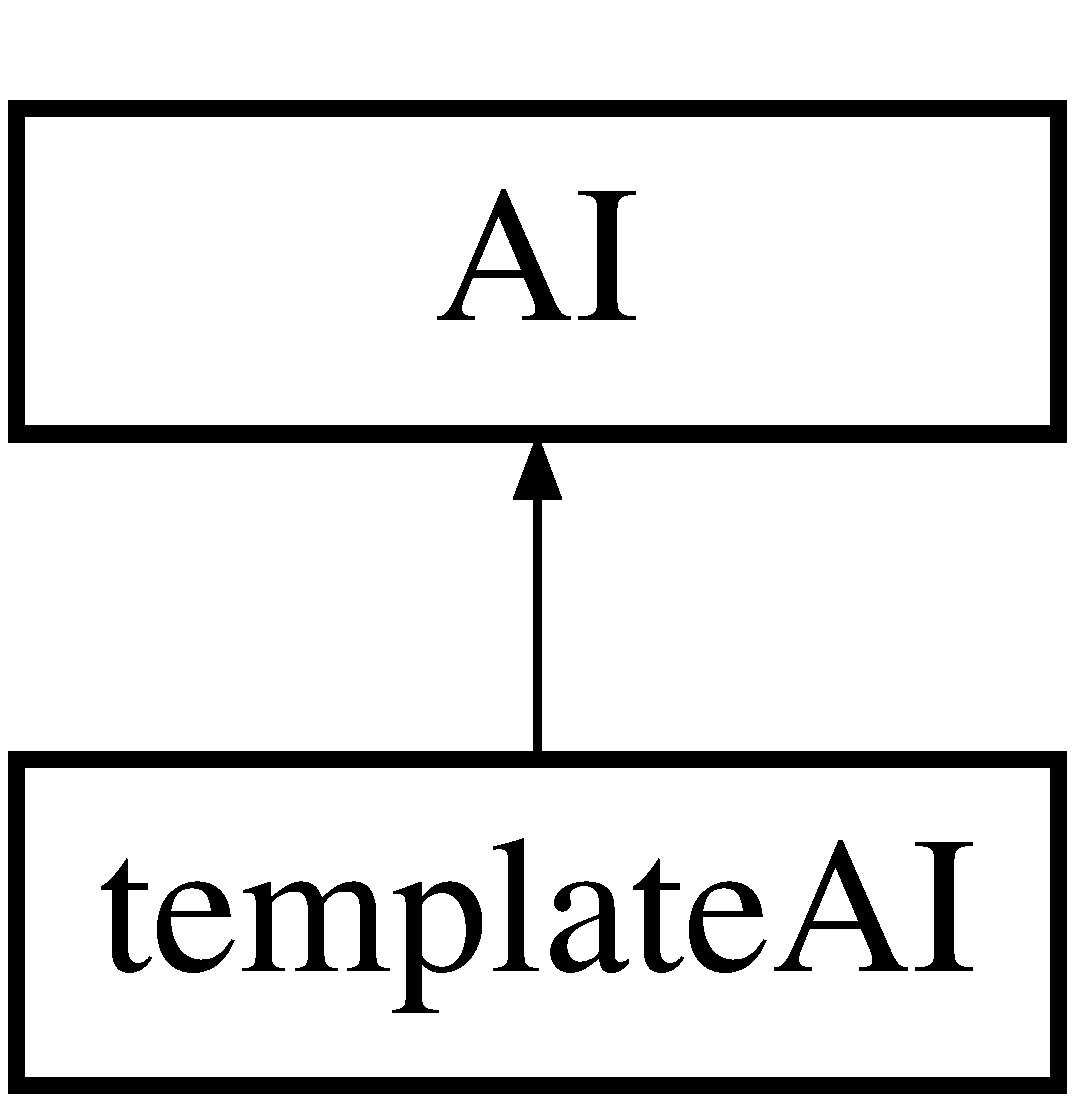
\includegraphics[height=2.000000cm]{classtemplate_a_i}
\end{center}
\end{figure}
\subsection*{Public Member Functions}
\begin{DoxyCompactItemize}
\item 
{\bfseries template\-A\-I} (P\-L\-A\-Y\-E\-R\-C\-O\-L\-O\-R {\bf player\-Color})\label{classtemplate_a_i_a419e693d985f701d2ec5a1d9237d24d8}

\item 
{\bf Move} {\bf do\-Move} ({\bf State} \&current\-State, vector$<$ {\bf Move} $\ast$ $>$ move\-List)
\item 
const {\bf Coordinate} $\ast$ {\bf set\-Pawn} ({\bf State} \&current\-State)
\item 
bool {\bf count\-Points} ({\bf State} \&current\-State, vector$<$ {\bf Connection} $\ast$ $>$ \&return\-Path)
\item 
void {\bf gather\-Information\-End\-Of\-Round} (const {\bf Round\-Logger} $\ast$information\-About\-Game)
\end{DoxyCompactItemize}
\subsection*{Additional Inherited Members}


\subsection{Detailed Description}
This is a template for your \doxyref{A\-I}{p.}{class_a_i}. Everywhere, where T\-O\-D\-O adpat appears, you have to insert your A\-Iname instead of \doxyref{template\-A\-I}{p.}{classtemplate_a_i}. For explanation of the methods, look into the A\-I-\/class documentation. Also you have to add this headerfile into the include-\/list in the file \char`\"{}hdr/ai/\-A\-I\-List.\-h\char`\"{}. 

\subsection{Member Function Documentation}
\index{template\-A\-I@{template\-A\-I}!count\-Points@{count\-Points}}
\index{count\-Points@{count\-Points}!templateAI@{template\-A\-I}}
\subsubsection[{count\-Points}]{\setlength{\rightskip}{0pt plus 5cm}bool template\-A\-I\-::count\-Points (
\begin{DoxyParamCaption}
\item[{{\bf State} \&}]{current\-State, }
\item[{vector$<$ {\bf Connection} $\ast$ $>$ \&}]{return\-Path}
\end{DoxyParamCaption}
)\hspace{0.3cm}{\ttfamily [virtual]}}\label{classtemplate_a_i_a254a3e1a7a2cd1d16bec816cb9fab075}
Here you can count your minus points at the end of each round. If you want to do so, you have to return true. For the beginning it is okay, if you just return false. Then the gamemaster will count the minuspoints. He counts in most cases the minimum of minuspoints you get, however in some cases the algorithm doesn't evaluate the best value. 

Implements {\bf A\-I} \doxyref{}{p.}{class_a_i_a158672aaf98fab1b1ede48002f83d3ff}.

\index{template\-A\-I@{template\-A\-I}!do\-Move@{do\-Move}}
\index{do\-Move@{do\-Move}!templateAI@{template\-A\-I}}
\subsubsection[{do\-Move}]{\setlength{\rightskip}{0pt plus 5cm}{\bf Move} template\-A\-I\-::do\-Move (
\begin{DoxyParamCaption}
\item[{{\bf State} \&}]{aktuell, }
\item[{vector$<$ {\bf Move} $\ast$ $>$}]{move\-List}
\end{DoxyParamCaption}
)\hspace{0.3cm}{\ttfamily [virtual]}}\label{classtemplate_a_i_a9abd9bfabeb26ba77ed5090cb1716a2a}
Inside this methode you calculate your next move in the game. 

Implements {\bf A\-I} \doxyref{}{p.}{class_a_i_ade352ac8d216d67feca731a127b50e6f}.

\index{template\-A\-I@{template\-A\-I}!gather\-Information\-End\-Of\-Round@{gather\-Information\-End\-Of\-Round}}
\index{gather\-Information\-End\-Of\-Round@{gather\-Information\-End\-Of\-Round}!templateAI@{template\-A\-I}}
\subsubsection[{gather\-Information\-End\-Of\-Round}]{\setlength{\rightskip}{0pt plus 5cm}void template\-A\-I\-::gather\-Information\-End\-Of\-Round (
\begin{DoxyParamCaption}
\item[{const {\bf Round\-Logger} $\ast$}]{current\-Infos}
\end{DoxyParamCaption}
)\hspace{0.3cm}{\ttfamily [virtual]}}\label{classtemplate_a_i_acfc0b92fbecc56c0dbde089c350f99e5}
At the end of each round you can take a look at the whole game and the playing cards of your opponents. This can be usefull, if you want to figure out there strategy and react to that over a simulation period. 

Implements {\bf A\-I} \doxyref{}{p.}{class_a_i_a8565a9ef04ac4f9913913c99f65213b2}.

\index{template\-A\-I@{template\-A\-I}!set\-Pawn@{set\-Pawn}}
\index{set\-Pawn@{set\-Pawn}!templateAI@{template\-A\-I}}
\subsubsection[{set\-Pawn}]{\setlength{\rightskip}{0pt plus 5cm}const {\bf Coordinate} $\ast$ template\-A\-I\-::set\-Pawn (
\begin{DoxyParamCaption}
\item[{{\bf State} \&}]{aktuell}
\end{DoxyParamCaption}
)\hspace{0.3cm}{\ttfamily [virtual]}}\label{classtemplate_a_i_ae18d50c605f126fc1d340368a76574bb}
At the beginning of each round you have to define your starting position of your pawn. 

Implements {\bf A\-I} \doxyref{}{p.}{class_a_i_a06aa99d4b4ac2530dbdad122183600e8}.



The documentation for this class was generated from the following files\-:\begin{DoxyCompactItemize}
\item 
hdr/ai/template\-A\-I.\-h\item 
src/ai/template\-A\-I.\-cpp\end{DoxyCompactItemize}

\section{Vector Class Reference}
\label{class_vector}\index{Vector@{Vector}}


{\ttfamily \#include $<$Vector.\-h$>$}

Inheritance diagram for Vector\-:\begin{figure}[H]
\begin{center}
\leavevmode
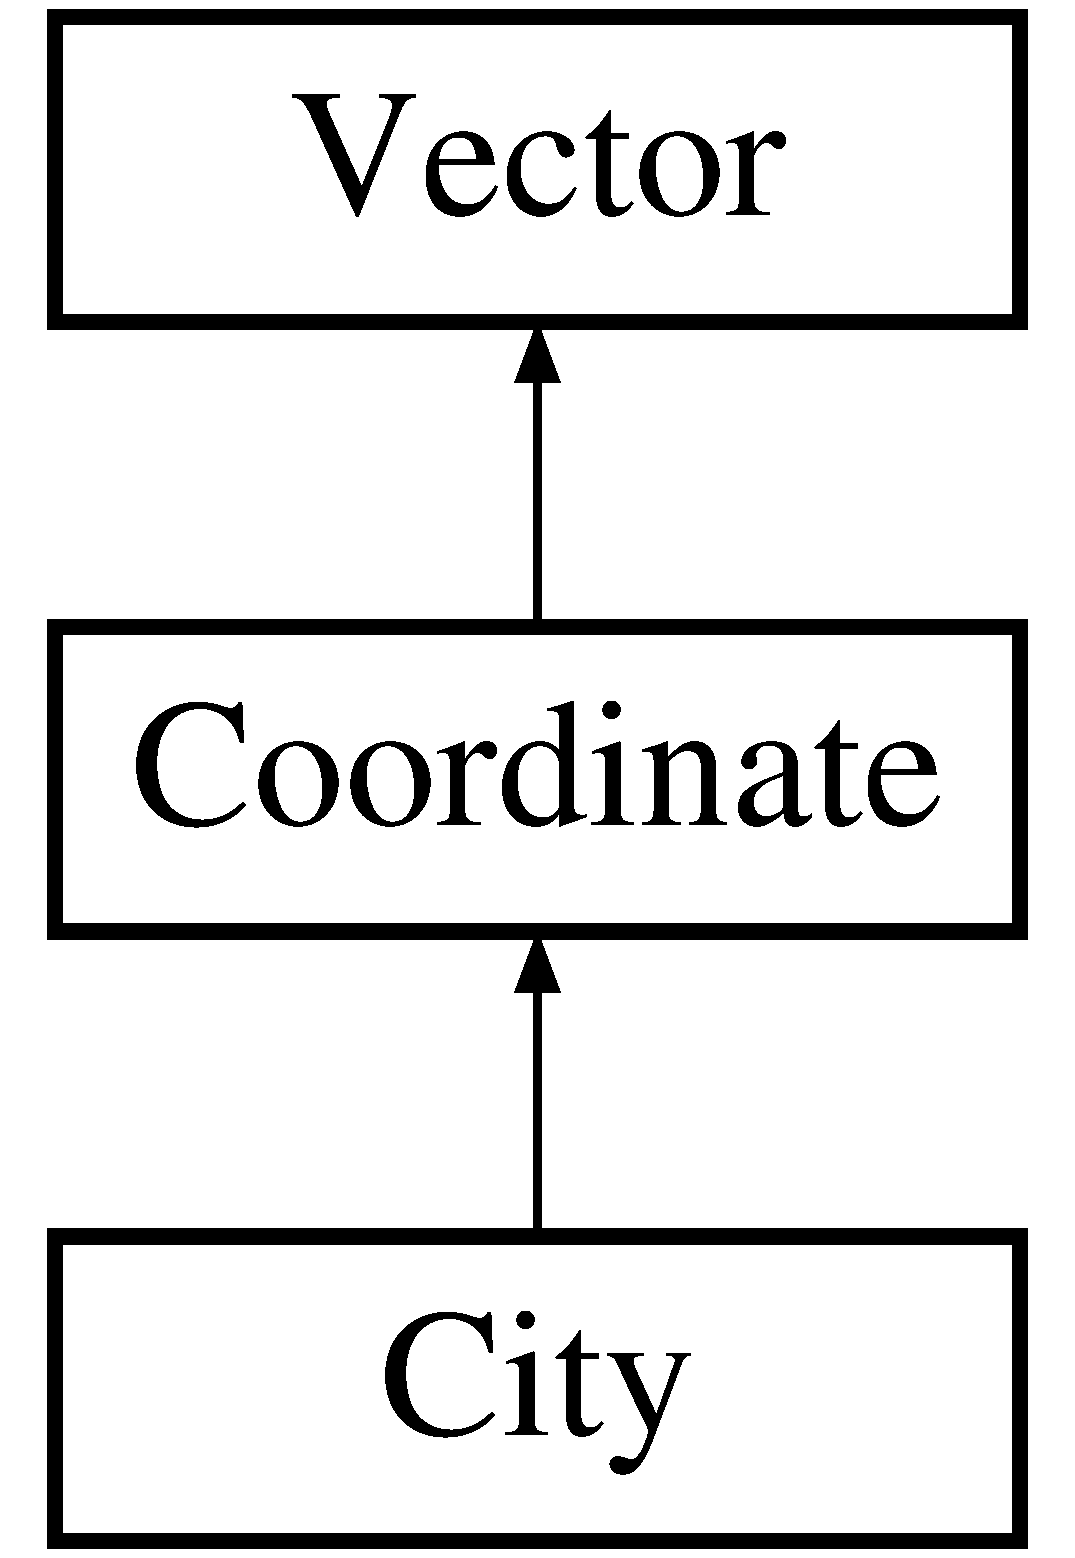
\includegraphics[height=2.000000cm]{class_vector}
\end{center}
\end{figure}
\subsection*{Public Member Functions}
\begin{DoxyCompactItemize}
\item 
{\bfseries Vector} (short x, short y)\label{class_vector_adbd8debb014cdfb97224a1d57b8d44a6}

\item 
{\bf Vector} {\bfseries operator-\/} (const {\bf Vector}) const \label{class_vector_aa283b61aaf9c0895288df72a56ac8899}

\item 
{\bf Vector} {\bfseries operator+} (const {\bf Vector}) const \label{class_vector_aad6d0d53c60571b1bbc52f1ecbc7b0c0}

\item 
short {\bf distance} () const 
\item 
void {\bf dump} () const 
\end{DoxyCompactItemize}
\subsection*{Public Attributes}
\begin{DoxyCompactItemize}
\item 
short {\bfseries x}\label{class_vector_a6784dd08f2e63d06fd376ddaa641f54c}

\item 
short {\bfseries y}\label{class_vector_a17bf7f9707a6ba166c08472377c8c732}

\end{DoxyCompactItemize}


\subsection{Detailed Description}
An object of the class \doxyref{Vector}{p.}{class_vector} represents a 2-\/dimensional vector with two integer values. It is a vector referenced to the board of the game. 

\subsection{Member Function Documentation}
\index{Vector@{Vector}!distance@{distance}}
\index{distance@{distance}!Vector@{Vector}}
\subsubsection[{distance}]{\setlength{\rightskip}{0pt plus 5cm}short Vector\-::distance (
\begin{DoxyParamCaption}
{}
\end{DoxyParamCaption}
) const}\label{class_vector_ac57f428cc1e03ce8cd3c9f6c98a8336f}
Determines a non-\/negative integer, that represents the distance on the board in terms of steps. \-: This distance doesn't represent the number of steps, because it doesn't take care of bridges/tunnels! \index{Vector@{Vector}!dump@{dump}}
\index{dump@{dump}!Vector@{Vector}}
\subsubsection[{dump}]{\setlength{\rightskip}{0pt plus 5cm}void Vector\-::dump (
\begin{DoxyParamCaption}
{}
\end{DoxyParamCaption}
) const\hspace{0.3cm}{\ttfamily [inline]}}\label{class_vector_a50123df9754e508f3d4aa7cb72f38905}
Dumps the values of the vector on the standard stream. 

The documentation for this class was generated from the following files\-:\begin{DoxyCompactItemize}
\item 
game/header/Vector.\-h\item 
game/source/Vector.\-cpp\end{DoxyCompactItemize}

%--- End generated contents ---

% Index
\newpage
\phantomsection
\addcontentsline{toc}{chapter}{Index}
\printindex

\end{document}
